%\documentclass[11pt, oneside]{article}       % use "amsart" instead of "article" for AMSLaTeX format
\documentclass[twocolumn]{svjour3}       % Spring article format
\journalname{Journal of Computational Neuroscience}
\usepackage[utf8]{inputenc}
\usepackage{microtype}

\usepackage{geometry}                        % See geometry.pdf to learn the layout options. There are lots.
\geometry{letterpaper}                           % ... or a4paper or a5paper or ...
%\geometry{landscape}                        % Activate for for rotated page geometry
%\usepackage[parfill]{parskip}            % Activate to begin paragraphs with an empty line rather than an indent
\usepackage{graphicx}                % Use pdf, png, jpg, or eps with pdflatex; use eps in DVI mode
                                % TeX will automatically convert eps --> pdf in pdflatex
\usepackage{amssymb}
\usepackage{amsmath}
\usepackage{mathptmx} % times font, as per journal
\usepackage{subfig}   % subfigure labeling (e.g., 1a)
\usepackage{float}    % adds the "H" placement option to force the figure to be inline
\usepackage{natbib}
\usepackage{multirow}
\usepackage{rotating}
\usepackage{array}
\usepackage{fixltx2e} % fix two column figure order
%\usepackage[textsize=tiny]{todonotes}
\usepackage[disable]{todonotes}
\usepackage{draftwatermark} % mark this as a draft

% centered overlap used to allow the expression for the summation range (under
% the sigma to extend under other parts of the equation.
% from Perlis, TUGboat Vol 0, no 0, 2001
\def\clap#1{\hbox to 0pt{\hss#1\hss}}
\def\mathclap{\mathpalette\mathclapinternal}
\def\mathllap{\mathpalette\mathllapinternal}
\def\mathrlap{\mathpalette\mathrlapinternal}
\def\mathclapinternal#1#2{\clap{$\mathsurround=0pt#1{#2}$}}
\def\mathllapinternal#1#2{\llap{$\mathsurround=0pt#1{#2}$}}
\def\mathrlapinternal#1#2{\rlap{$\mathsurround=0pt#1{#2}$}}

\renewcommand{\topfraction}{0.9} % allow more floats to fill most of the page
\renewcommand{\dbltopfraction}{0.9} % as above, but in 2 column mode

% typing shortcuts

% short author and title for top of page (Springer specific)

\titlerunning{Dynamical Architecture for Adaptive Responses to Mechanical Loads}
\authorrunning{Shaw KM, Cullins MJ, McManus JM, Lu H, Thomas PJ, Chiel HJ}

\title{The Significance of Dynamical Architecture for Adaptive Responses to Mechanical Loads During Rhythmic Behavior}
\author{
    Kendrick M.~Shaw \and Miranda J.~Cullins \and Jeffrey M.~McManus \and Hui Lu \and Peter J.~Thomas \and Hillel J.~Chiel}
%\date{}                            % Activate to display a given date or no date


\newlength{\figwidth}
\figwidth=\linewidth
\let\ifthesis=\iffalse


\institute{
    Kendrick M.~Shaw \at
    Department of Biology and Medical Scientist Training Program, Case Western Reserve University, 10900 Euclid Ave., Cleveland OH 44106, USA \\
    \email{kendrick.shaw@case.edu}           %  \\
    \and
    Miranda J.~Cullins $\cdot$ Jeffrey M.~McManus $\cdot$ Hui Lu \at
    Department of Biology, Case Western Reserve University, 10900 Euclid Ave., Cleveland OH 44106, USA
    \and
    Peter J.~Thomas \at
    Departments of Mathematics, Biology and Cognitive Science, Case Western Reserve University, 10900 Euclid Ave., Cleveland OH 44106, USA \\
    \email{peter.j.thomas@case.edu}           %  \\
    \and
    Hillel J.~Chiel \at
    Departments of Biology, Neurosciences and Biomedical Engineering, Case Western Reserve University, 10900 Euclid Ave., Cleveland OH 44106, USA \\
    \email{hjc@case.edu}           %  \\
}

\date{Received: date / Accepted: date}
% The correct dates will be entered by the editor


\begin{document}
\listoftodos
\maketitle

\begin{abstract}
Many behaviors require reliably generating sequences of motor activity while
adapting the activity to incoming sensory information.  This process has often
been conceptually explained as either fully dependent on sensory input (a
chain reflex) or fully independent of sensory input (an idealized central
pattern generator, or CPG), although the consensus of the field is that most neural
pattern generators lie somewhere between these two extremes.  Many mathematical
models of neural pattern generators use limit cycles to generate the sequence
of behavior, but other models, such as a heteroclinic channel (an attracting
chain of saddle points), have been
suggested.  To explore the continuum between CPGs and chain reflexes, in this
paper we describe a nominal model of feeding in
\textit{Aplysia californica} that can be smoothly shifted between a
generic limit cycle (where the velocity changes by less than an order of
magnitude throughout the cycle) and a heteroclinic channel (where the velocity
becomes small when the trajectory passes near saddle points).  We then study
the behavior of the system in these two parameter regimes and compare the
behavior of the models with behavior recorded in the animal \textit{in vivo}
and \textit{in vitro}.  We show that while both pattern generators can generate
similar behavior, the stable heteroclinic channel can better respond to
small changes in sensory input induced by load, and that the response matches
the changes seen when a load is added \textit{in vivo}.  We then show that
the stable heteroclinic channel shows much more dramatic slowing of activity
than the generic limit cycle when sensory input is reduced, and show that
similar slowing with removal of proprioception is seen \textit{in vitro}.
Finally, we show that the distributions of burst lengths seen \textit{in
vivo} are better matched by the distribution expected from a stable
heteroclinic channel than that expected from a generic limit cycle.
These observations suggest that feeding behavior in \textit{Aplysia} may be
better described by a model using a heteroclinic channel than a more generic
limit cycle.

\keywords{Aplysia \and heteroclinic channel \and Central Pattern Generator \and Chain reflex \and Limit cycle}
% \PACS{PACS code1 \and PACS code2 \and more}
% \subclass{MSC code1 \and MSC code2 \and more}
\end{abstract}

\newlength\desccolwidth
\newlength\varcolwidth

\section{Introduction}

Motor behaviors, such as cat running, crayfish swimming, and dog lapping all
require the nervous system to reliably generate a sequence of motor outputs.
To be efficient, however, a fixed sequence of activity is not enough: a cat
that fails to step over an obstacle may lose its footing and fall
\citep{forssberg_phase_1975,forssberg_stumbling_1979}
and a crayfish that wanders into a
current of cold water must control muscles that may suddenly have become
stronger but relax more slowly \citep{harri_effects_1977}.  Sensory
feedback plays a key role in allowing an animal to adapt its behavioral pattern
to the circumstances in which it finds itself.  The way that this sensory
information is integrated into pattern generation to produce adaptive behavior,
however, can be difficult to ascertain.

Historically, two competing theories have been proposed for how the nervous
system can generate sequences of motor
activity \citep{marder_central_2001}.  At one extreme,
\citet{loeb_einleitung_1899} proposed that
sensory input is required for the transitions between behaviors, so that the
sequence of behavior is formed of a chain of reflexes each leading to the next.
He thus proposed calling this form of pattern generation a ``kettenreflex,'' or
``chain reflex.''  For example, during walking, this theory would predict that
extension of the leg continues until sensory input indicates that the foot has
struck the ground, and in the absence of this sensory input, the pattern would
not progress.  This theory was later elaborated by Sherrington, who noted that
bouts of walking-like movements could be evoked in the hind limbs of a dog
after spinal transection by dropping the limb, and these motor patterns would
stop abruptly when the limb was passively mechanically arrested
\citep{sherrington_flexion-reflex_1910}.

Even chain reflex theory's strongest advocates saw it as an incomplete
explanation of what was observed in the biology, however.  Sherrington, noting
that spinal stimulation could produce step-like movements even in a
deafferented limb, concluded ``These difficulties suggest that generation of a
secondary local stimulus and its interference with the operation of the primary
remote stimulus, although regulative of the rhythm (cf. vagus and respiratory
rhythm) is of itself not the sole rhythm-producing factor in the reflex.'' By
the time Wilson showed that the nervous system in the locust could generate
strong structured motor patterns in the absence of sensory input
\citep{wilson_central_1961}, investigators had come to assume that sequences of
motor activity were primarily generated by a central pattern generator.  The
central pattern generator theory suggests that the nervous system can, on its
own, produce appropriate patterns of motor activity even in the absence of
sensory input. At best, sensory input merely serves to modulate this underlying
neural pattern.

It should be noted, however, that patterns generated by the isolated nervous
system often are very distorted compared to those seen \textit{in vivo}.  In
particular, phases of the motor pattern are often significantly longer than
those observed in the intact animal. \todo{"For example XXX" cite numbers for
locust flight, crayfish swimmerets, lamprey, rat?}  This has led many
investigators to question the descriptive power of central pattern generator
theory. In the words of Robertson and Pearson, ``Although now abundantly clear
that a central rhythm generator can produce powerful oscillations in the
activity of flight motor neurons and interneurons, it is equally clear that the
properties of this central oscillator cannot fully account for the normal
flight pattern'' \citep{selverston_model_1985}.

There is some evidence that slowing of isolated neural patterns may be due to
the absence of sensory feedback.  In \citet{pearson_phase-dependent_1983}, cycle-by-cycle
stimulation of the appropriate sensory afferents was able to restore wing-beat
frequency in fictive flight in the locust.  \todo{(cite crayfish group from
Neuroethology) have shown similar results in crayfish swimmeret activity.}
Restoration of the normal pattern by sensory input suggests that biological
pattern generators may occupy a middle ground between pure central pattern
generators and chain reflexes.  In some cases, endogenous neural input may
control where a systems lies on this continuum.   As
\citet{bassler_definition_1986} noted when considering a relaxation-oscillator
like model of a central pattern generator ``Hence, one and the same system can
behave either like a CPG or like a chain reflex, depending only on the amount
of endogenous input.''  These investigators thus warned about the dangers of inferring the
mechanism used by a pattern generator \textit{in vivo} based only on the
behavior of a pattern generator \textit{in vitro}.

Despite these hesitations, the empirical data supporting central pattern
generator hypothesis led to a focus on providing a mathematical formulation
for this theory using the qualitative analysis of dynamical
systems, which was becoming an important tool for theoretical neuroscience by
the middle of the twentieth century. The behavior of an ideal central pattern
generator naturally corresponds to a system of nonlinear ordinary differential
equations whose solutions contain stable limit cycle (an attracting isolated
periodic orbit).  As a result, this structure has played a central role in the
mathematical description of central pattern generators
\citep{ijspeert_central_2008}.
\todo{cite Koppel 1986?  PJT - was this meant to
    be the chapter from "Neurobiology of vertebrate locomotion" or the paper
    "Coupled Oscillators and Locomotion by Fish" \citep{kopell_coupled_1986}?
    Case does not have access/copies of either, but I've requested both via
    Ohiolink}

In contrast, there have been fewer attempts to model chain reflexes with
systems of differential equations.  Instead, much of the work modeling
these types of sensory-dependent systems use different tools, such as
finite state machines \citep{lewinger_sensory_2006}.  While these models can capture individual phases of the behavior well,
they generally do not describe the transitions between the phases, which may
be important in understanding some forms of behavior.  In contrast, one could
view the state of a chain reflex system in terms of a series of stable fixed
points.  In each phase of the motion,
the trajectory would be captured by one of the fixed points until the
appropriate (external) sensory input pushed the system out of the neighborhood
attracted to that fixed point and into the basin of attraction of the next.

Between these two extremes of models of central pattern generators and chain
reflexes, one may consider systems in which the progress of a periodic orbit is
slowed, but not stopped, by passage near one or more fixed points.  This
behavior arises naturally in a structure known as a ``stable heteroclinic channel''
\citep{rabinovich_transient_2008}, where multiple saddle points (fixed points
that attract in some directions while repelling in others) are connected in a
cycle, so that the unstable manifold of each saddle point brings
the system near the stable manifold of the next fixed point.  This structure has been used
to describe motor behavior such a predatory swimming behavior in
\textit{Clione} \citep{levi_dual_2004,varona_competing_2004}.
\todo{ and ...(fill in cites from Rabinovich et al)}  To our
knowledge, however, these models of pattern generation have not been directly
compared to those built with a more ``pure'' limit cycle that does not pass near
fixed points.

A potential advantage of a dynamical system that allows trajectories to move close
to equilibrium points is that it may spend longer or shorter times in that vicinity,
rather than proceeding through the cycle with a relatively fixed phase velocity.
In turn, this could allow an animal greater flexibility in responding to unexpected
changes in the environment, such as increases or decreases in mechanical load as it
attempts to manipulate an object.

To examine this range of dynamics, we have created a neuromechanical model
based on the feeding apparatus of the marine mollusk \textit{Aplysia
californica}.  We examine the model in two parameter regimes which produce
similar output under small loads.  In the first parameter regime, the isolated
neural dynamics form a homogeneous limit cycle, as would be expected for an
idealized central pattern generator.  In the second parameter regime, the
isolated neural dynamics form a stable heteroclinic cycle, moving it closer
along the continuum to a chain reflex.  We show that in
this second regime, the behavior of the model falls between that of an
idealized chain reflex and an idealized central pattern generator.  We then
compare the behavior of the two models to the observed behavior of the animal,
and show that several of the features of the animal's behavior are better
described by the model with the stable heteroclinic channel than the
model with the limit cycle.  At the end of the paper, we reflect on
possible general principles suggested by this work.

\section{Mathematical Framework}
\label{sec:mathematical_framework}

In this section we describe a general mathematical framework we will use for
modeling the behavior of motor pattern generators.  We model a central pattern
generator receiving sensory input from the body as a system of
differential equations specifying the evolution of a vector of $n$ neural state
variables, $a \in \mathbb{R}^n$, and a vector of $m$ state variables, $x \in
\mathbb{R}^m$, representing the mechanics and periphery (e.g. muscle
activation).  We assume that an applied load interacts only with the
mechanical state variables, so that the differential equations can be
naturally written in the following form:
\begin{align}
    \frac{da}{dt} &= f(a, \mu) + \epsilon g(a, x),\label{eq:generic_a}\\
    \frac{dx}{dt} &= h(a, x) + \kappa l(x).\label{eq:generic_x}
\end{align}
Here $\mu$ is a vector of parameters which can encode states such as arousal
of the animal, $f(a, \mu)$ represents the intrinsic dynamics of a motor
pattern pattern generator, $h(a, x)$ represent the dynamics of the periphery
with the given central input, $g(a, x)$ represents the effects of sensory
feedback from the periphery, $l(x)$ represents the effects of an external
load or perturbation, and $\epsilon, \kappa \in \mathbb{R}^+$ are scaling
constants, not necessarily small.  We further assume that all of these
functions are smooth, infinitely differentiable, and have bounded ranges over
the domain of interest.

\subsection{Limit cycles}

We first consider the case of an idealized central pattern generator, where a
part of the nervous system can produce sequences of motor activity that closely
resemble those seen \textit{in vivo}, even when it is not attached to the
periphery.  Thus we assume that, for some range of the parameter $\mu$,
the dynamics of the isolated neural circuit,
$da/dt = f(a, \mu)$, contain an attracting limit cycle $\gamma(t)$ which
represents the observed motor pattern.  We make the further important
assumption that there exists a behaviorally relevant mechanical load
$\kappa l(x)$ with which the complete system contains a corresponding limit
cycle $\xi(t)$, such that the neural component of $\xi(t)$ closely matches that
of the isolated system.  By this we mean that, with appropriately chosen
initial conditions,
\begin{equation}
    \int_0^T ||\gamma(t) - P_a \xi(t)||^2\;dt \ll 1,
    \label{eq:CPG_error}
\end{equation}
where $P_a : \mathbb{R}^{m+n} \to \mathbb{R}^n$ is the projection operator onto
the $a$ subspace, $T$ is the period of $\gamma(t)$, and $||\cdot||$ is the
usual $L^2$ (Euclidean) norm.  Note that it is possible that these very similar
patterns will produce very different behavior in the periphery.  Therefore, we
will also assume that this isolated pattern
$\gamma(t)$ produces similar behavior in the periphery, that is that the system
$dx/dt = h(\gamma(t), x) + \kappa l(x)$ contains an attracting periodic orbit
$\zeta(t)$ such that with an appropriate choice of initial conditions
\begin{equation}
    \int_0^T ||\zeta(t) - P_x \xi(t)||^2\;dt \ll 1,
    \label{eq:CPG_periph_error}
\end{equation}
where $P_x : \mathbb{R}^{m+n} \to \mathbb{R}^m$ is the projection operator onto
the $x$ subspace.  Finally, we assume that gradually adding back sensory input
does not distort the pattern or the behavior, meaning that both $\gamma(t)$ and
$\zeta(t)$ persist for small values of $\epsilon$ and remain similar to
projections of $\xi(t)$.

Because the system is smooth, the integral in (\ref{eq:CPG_error})
can be made to be small by insuring that the magnitude of the sensory feedback,
$||\epsilon g(P_a \xi(t), P_x \xi(t))||$, is small for all $t \in (0,
T)$\todo{I'd like an "if and only if", but large high-frequency changes can be
filtered out.  Is there a clean way to exclude those?}.  Although a careful
choice of $||g||$ could be small along $\xi$ but not elsewhere, we will focus
on the more generic case where $\epsilon \ll 1$.

\subsection{Destabilization of fixed points}
\label{sec:chain_reflex}

We next consider the chain reflex.  In this case the dynamics of the isolated
nervous system, $da/dt = f(a, \mu)$, will contain a set of stable nodes, $A$,
where each node represents a ``stage'' of the chain reflex, that can be
destabilized by sensory input.  Note that in this case, unlike the central
pattern generator, $\epsilon$ may need to be of $O(1)$ to destabilize a node.
The combined dynamics of the nervous system and the periphery, however, would
still be expected to contain a stable limit cycle $\xi(t)$ rather than a series
of fixed points.  Similar dynamics have been seen in models of other biological
oscillators; for example in \citet{novak_model_1998} the authors created a
model of the cell cycle where fixed points in the biochemical dynamics
(analogous to the isolated neural dynamics) can be destabilized by changes in
cell size (analogous to the periphery) so that the coupled system contains a
limit cycle.  Because a chain reflex can not explain the fictive motor patterns
produced by the isolated nervous system, we will not explore this alternative in
in this paper.

\subsection{Stable heteroclinic channels}
We now consider a system that is intermediate between the two extremes of an
idealized central pattern generator and a chain reflex.  We can construct
such a system from a set of $n$-dimensional hyperbolic saddle points, each with a
one-dimensional unstable manifold and an $n-1$ dimensional stable manifold,
arranged in a cycle such that the unstable manifold of one saddle point
intersects the stable manifold of the next, forming a heteroclinic orbit.  We
refer to these saddle points and their connecting heteroclinic orbits as a
\emph{heteroclinic cycle} \citep{guckenheimer_structurally_1988}.

Under appropriate conditions, this heteroclinic cycle attracts nearby orbits
(and thus can be called a stable heteroclinic cycle).  In particular, if we
define the (positive) ratio of the least negative stable eigenvalue
$\lambda_{i,\textrm{s}}$ and the unstable eigenvalue $\lambda_{i,\textrm{u}}$
of the $i$th saddle as the saddle index $\nu_i = -\lambda_{i,\textrm{s}} /
\lambda_{i,\textrm{u}}$ \citep{shilnikov_methods_2002}, then the heteroclinic
cycle will attract nearby orbits if $\prod_i \nu_i > 1$
\citep{afraimovich_heteroclinic_2003}.  This type of dynamics can arise
naturally from neural models involving symmetric mutually inhibitory pools of
neurons; for example see \citet{nowotny_dynamical_2007}.

An unperturbed trajectory on the
heteroclinic cycle will, like the chain reflex model in
section~\ref{sec:chain_reflex}, asymptotically approach a fixed point.
Unlike the chain reflex model, however, a very small perturbation in the
unstable direction will push the trajectory out of the stable manifold,
allowing the trajectory to leave the neighborhood of the fixed point (and
potentially travel to the neighborhood of the next fixed point).  Arbitrarily
small amounts of noise can thus insure that the system will almost certainly
not remain stuck at a given fixed point \citep{stone_random_1990}.  Thus,
rather than the stability of states seen in the chain reflex model, the
heteroclinic cycle exhibits metastability \citep{afraimovich_nonlinear_2011},
where the trajectory spends long but finite periods of time near each fixed
point \citep{bakhtin_noisy_2011}.
Thus, like the chain reflex, the system can spend short or long periods of time
in one particular state depending on sensory input, but, like the limit cycle,
the system will eventually transition to the next state even in the absence of
sensory input.

While stable heteroclinic cycles are structurally unstable (i.e. a small
change in the vector field will generally break the cycle), small
perturbations can result in the creation of a stable limit cycle that
passes very close to the saddles.  For example, in the planar case, any
sufficiently small perturbation that pushes the unstable manifold of the
saddles towards the inside of the unperturbed stable heteroclinic cycle will
result in a stable limit cycle \citep{reyn_generation_1980}.  Similar
conditions can be found for higher dimensional stable heteroclinic cycles
\citep{afraimovich_heteroclinic_2003}.  These families of limit cycles
that pass close to the original saddles, known as stable heteroclinic
channels \citep{rabinovich_transient_2008}, are structurally stable, and
exhibit many of the same properties of sensitivity and metastability as the
original stable heteroclinic cycles.  As we will see, this extreme sensitivity
can be advantageous for generating adaptive behaviors.

In the next section we provide an example of model dynamics $f(a,\mu)$
exhibiting a limit cycle for $\mu>0$ and a bifurcation to a heteroclinic
cycle at $\mu=0$.  We then investigate the behavior of the full $(a,x)$ system
in the ``limit cycle'' and ``heteroclinic cycle'' parameter regimes.

\section{Model Description}
\label{sec:model_description}

\subsection{Neural model}
\label{sec:neural_model}

We wish to explore the effects of different types of neural dynamics on the
behavior of the animal.  Although detailed, multi-cellular and
multi-conductance models of neurons and circuits underlying feeding pattern
generation in \textit{Aplysia} have been described \citep{baxter_feeding_2006,
cataldo_computational_2006, susswein_mechanisms_2002}, the complexity of these
models makes it difficult to use them for mathematical analysis.  As a
consequence, we choose to represent motor pools (which contain neurons that are
electrically coupled to one another or have mutual synaptic excitation) using
nominal firing-rate models.

As discussed in section~\ref{sec:mathematical_framework}, we define the neural
dynamics as a combination of an intrinsic component, $f(a, \mu)$, that does
not depend on the periphery, and a sensory (coupling) component, $g(x)$, which
does depend on the periphery.  For mathematical tractability, we assume that
the intrinsic and sensory drive combine linearly, thus giving the evolution
equation of the neural activity.
\begin{equation}
\label{eq:neural_dynamics}
\frac{da}{dt} = f(a, \mu) + \epsilon g(x_\textrm{r}),
\end{equation}
where $a$ is a vector of the activity of each of the $N$ neurons, $\epsilon$
is a parameter scaling the strength of sensory input, $x_\textrm{r}$ is
a biomechanical state variable which we will define in more detail in
section~\ref{sec:periphery_model}, and $\mu$ is a parameter that can shape
the intrinsic dynamics.  Specifically we will consider the following
modified Lotka--Volterra model which captures the dynamics of $N$ neural pools:
\begin{equation}
    \label{eq:f_def_generic}
    f_i(a,\mu) = \frac{1}{\tau_\textrm{n}}\left(\left(1 - \sum_j \rho_{ij} a_j \right) a_i + \mu\right),
\end{equation}
for $0 \le i < N$.
Here $\mu$ is a scalar parameter
representing intrinsic excitation, $\tau_\textrm{n}$ is a time constant, and $\rho$ is the
coupling matrix
\begin{equation}
    \rho_{ij} = \left\{\begin{array}{c@{\qquad}l}
        1 & i = j \\
        0 & i = j - 1 \pmod{N} \\
        \gamma & \textrm{otherwise},
    \end{array}\right.
\end{equation}
where $\gamma$ is a coupling constant representing inhibition between neural
pools.
\todo{update code to use new names for $tau_a \to \beta$, $tau_l \to \alpha$, $g \to \phi$, $\epsilon$, $x_o$ -> $x_\textrm{r}$}

\begin{figure}
    \centering
    \includegraphics[width=0.8\linewidth]{fig/lc_shc_sigma0_phaseplot}
    \caption[Isolated trajectories of the SHC and limit cycle]{
        When $\mu = 0$, in the absence of sensory input ($\epsilon =
        0$), the intrinsic neural dynamics contain a stable heteroclinic cycle
        (black line) connecting saddles at $(1,0,0)$, $(0,1,0)$, and $(0,0,1)$.
        When $\mu$ is a small positive number and $\epsilon = 0$, the
        heteroclinic cycle is broken and a stable limit cycle arises (shown in
        light blue for the value of $\mu$ used for the limit cycle in this
        paper).
    }
    \label{fig:lc_and_shc_phaseplot}
\end{figure}

\todo{As has been thoughly examined by Rabinovich, Afraimach...} When $N > 2$
and $\gamma > 2$ this system contains a stable heteroclinic cycle when $\mu =
0$.  In contrast, as shown in figure~\ref{fig:lc_and_shc_phaseplot}\todo{Figure: panel 1: 3D plot with
isolated stable heteroclinic channel and limit cycle, points indicating starting points half-way
between saddles.  Panel 2: time series plot of two points on the stable heteroclinic channel with limit
cycle and mu}, it contains a stable limit cycle for small positive values of
$\mu$, with the distance between the limit cycle and saddles increasing with
increasing values of $\mu$.  With the goal of parsimony, we use
$N = 3$ and thus (\ref{eq:f_def_generic}) can be expanded to
\begin{align}
    f_0(a, \mu) &= \frac{1}{\tau_\textrm{n}}(a_0 (1 - a_0 - \gamma a_1) + \mu),\\
    f_1(a, \mu) &= \frac{1}{\tau_\textrm{n}}(a_1 (1 - a_1 - \gamma a_2) + \mu),\\
    f_2(a, \mu) &= \frac{1}{\tau_\textrm{n}}(a_2 (1 - a_2 - \gamma a_0) + \mu).
\end{align}
We explain the correspondence of these three neural pools to neural
pools in \textit{Aplysia} in the next section.


\subsection{Model of the periphery and load}
\label{sec:periphery_model}
\begin{figure}
    \centering
    \ifthesis
        \figwidth=0.7\linewidth
    \else
        \figwidth=\linewidth
    \fi
    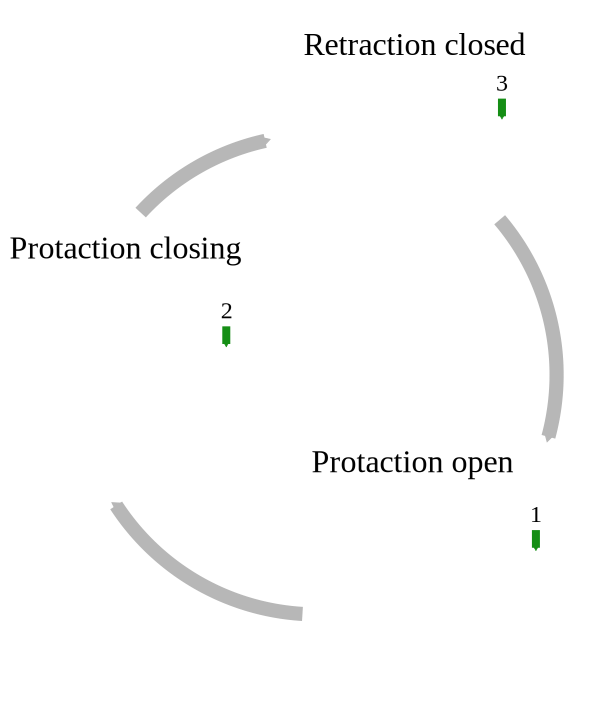
\includegraphics[width=\figwidth]{diagrams/model_storyboard}
    \caption[Phases of swallowing behavior in the model]{
         The model breaks swallowing into three phases.
         First, the odontophore protracts while open (lower right).
         Near the end of protraction, the odontophore begins closing
         (left) and protracts a small distance while closed.  In the last
         phase, the odontophore retracts while closed (upper right).
         The protraction muscle (I2) is shown in blue, the grasper
         (the radula-odontophore) is shown in red, and the
         ring-like retraction muscle (I3) is shown in yellow,
         with a section cut away to show the grasper.  The green
         strand is seaweed, with the arrows showing how the seaweed moves
         within a single cycle.}
    \label{fig:model_storyboard}
\end{figure}
\begin{figure}
    \centering
    \ifthesis
        \figwidth=0.7\linewidth
    \else
        \figwidth=\linewidth
    \fi
    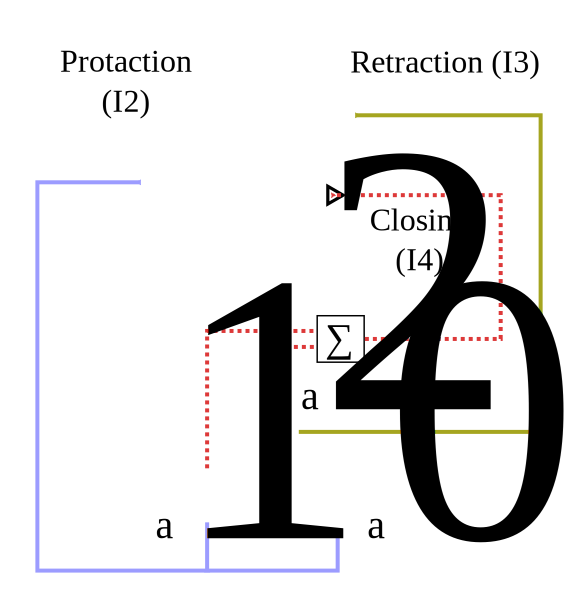
\includegraphics[width=\figwidth]{diagrams/model_diagram}
    \caption[Model schematic]{
        Schematic of the neuromechanical model of the feeding apparatus
        in \textit{Aplysia}.  The three neural pools ($a_0$, $a_1$, and $a_2$)
        control three phases of the behavior shown in figure
        \ref{fig:model_storyboard}: protraction open, protraction closing, and
        retraction closed.  The solid lines and triangles indicate excitatory synaptic
        coupling with a neuromuscular transform represented by a low pass
        filter.  The dashed line and summation symbol represent a simple
        summation and thresholding that control closing in the model.  The
        $a_0$ neural pool represents the B31, B32, and B63 neurons, the $a_1$ motor
        pool represents these same neurons with the addition of B8 (which experiences
        slow excitation from B34), and the $a_2$ motor pool represents B64, B3, B6, B9,
        and B8 (which is excited by B64) activity.}
    \label{fig:model_diagram}
\end{figure}

\ifthesis
\desccolwidth=100mm
\else
\desccolwidth=35mm
\fi
% params.tex
% generated from settings.yaml using ./yaml2tex
% on Thu Aug 29 15:15:29 2013


% model parameter values:
\newcommand{\paramValumax}{$1$}
\newcommand{\paramValsigmaITwo}{$-2\cdot10^{-3}$}
\newcommand{\paramValsigmah}{$2\cdot10^{-3}$}
\newcommand{\paramValsigmaIThree}{$2\cdot10^{-3}$}
\newcommand{\paramValgamma}{$2.4$}
\newcommand{\paramValxspring}{$0.9$}
\newcommand{\paramValbeta}{$1$}
\newcommand{\paramValkspring}{$0$}
\newcommand{\paramValalpha}{$1$}
\newcommand{\paramValdelta}{$0$}
\newcommand{\paramValFsw}{$0.01$}
\newcommand{\paramValmu}{$0$}
\newcommand{\paramValeta}{$0$}
\newcommand{\paramValtaua}{$0.05$}
\newcommand{\paramValtaulITwo}{$0$}
\newcommand{\paramValtaulh}{$0$}
\newcommand{\paramValtaulIThree}{$0$}
\newcommand{\paramValbo}{$0.1$}
\newcommand{\paramValkITwo}{$-1$}
\newcommand{\paramValkh}{$-1$}
\newcommand{\paramValkIThree}{$1$}
\newcommand{\paramValtau}{$2.45$}
\newcommand{\paramValSITwo}{$0.5$}
\newcommand{\paramValSh}{$0.5$}
\newcommand{\paramValSIThree}{$0.25$}
\newcommand{\paramValwITwo}{$2$}
\newcommand{\paramValwh}{$2$}
\newcommand{\paramValwIThree}{$1.1$}
\newcommand{\paramValcITwo}{$1$}
\newcommand{\paramValch}{$1$}
\newcommand{\paramValcIThree}{$1.1$}
\newcommand{\paramValaresetITwo}{$.nan$}
\newcommand{\paramValareseth}{$.nan$}
\newcommand{\paramValaresetIThree}{$.nan$}
\newcommand{\paramValbsw}{$0.10$}
\newcommand{\paramValtkick}{$150$}
\newcommand{\paramValxkick}{$0$}
\newcommand{\paramValakickITwo}{$0$}
\newcommand{\paramValakickh}{$0$}
\newcommand{\paramValakickIThree}{$0$}


% initial condition values:
\newcommand{\initValaIThree}{$10^{-9}$}
\newcommand{\initValah}{$10^{-9}$}
\newcommand{\initValaITwo}{$1.0$}
\newcommand{\initValxo}{$0.5$}
\newcommand{\initValxsw}{$0.0$}
\newcommand{\initValuITwo}{$0.0$}
\newcommand{\initValuIThree}{$0.0$}
\newcommand{\initValEITwo}{$0.0$}
\newcommand{\initValEIThree}{$0.0$}
\newcommand{\initValUITwo}{$0.0$}
\newcommand{\initValUIThree}{$0.0$}

% simulation parameter values:
\newcommand{\simParamValduration}{$300$}
\newcommand{\simParamValminOutputInterval}{$0.01$}
\newcommand{\simParamValdt}{$0.001$}
\newcommand{\simParamValseed}{$3235798765$}
\newcommand{\simParamValsweepSteps}{$1000$}


% parameter table example:

% \begin{tabular}[htb]{ccl}
%     parameter & value & description \\
%     \hline
%     $u_max$ & \paramValumax & \\
%     $\sigma_{I2}$ & \paramValsigmaITwo & \\
%     $\sigma_{h}$ & \paramValsigmah & \\
%     $\sigma_{I3}$ & \paramValsigmaIThree & \\
%     $\gamma$ & \paramValgamma & \\
%     $x_spring$ & \paramValxspring & \\
%     $\beta$ & \paramValbeta & \\
%     $k_spring$ & \paramValkspring & \\
%     $\alpha$ & \paramValalpha & \\
%     $\delta$ & \paramValdelta & \\
%     $F_sw$ & \paramValFsw & \\
%     $\mu$ & \paramValmu & \\
%     $\eta$ & \paramValeta & \\
%     $\tau_a$ & \paramValtaua & \\
%     $\tau_l_{I2}$ & \paramValtaulITwo & \\
%     $\tau_l_{h}$ & \paramValtaulh & \\
%     $\tau_l_{I3}$ & \paramValtaulIThree & \\
%     $b_o$ & \paramValbo & \\
%     $k_{I2}$ & \paramValkITwo & \\
%     $k_{h}$ & \paramValkh & \\
%     $k_{I3}$ & \paramValkIThree & \\
%     $\tau$ & \paramValtau & \\
%     $S_{I2}$ & \paramValSITwo & \\
%     $S_{h}$ & \paramValSh & \\
%     $S_{I3}$ & \paramValSIThree & \\
%     $w_{I2}$ & \paramValwITwo & \\
%     $w_{h}$ & \paramValwh & \\
%     $w_{I3}$ & \paramValwIThree & \\
%     $c_{I2}$ & \paramValcITwo & \\
%     $c_{h}$ & \paramValch & \\
%     $c_{I3}$ & \paramValcIThree & \\
%     $a_reset_{I2}$ & \paramValaresetITwo & \\
%     $a_reset_{h}$ & \paramValareseth & \\
%     $a_reset_{I3}$ & \paramValaresetIThree & \\
%     $b_sw$ & \paramValbsw & \\
%     $t_kick$ & \paramValtkick & \\
%     $x_kick$ & \paramValxkick & \\
%     $a_kick_{I2}$ & \paramValakickITwo & \\
%     $a_kick_{h}$ & \paramValakickh & \\
%     $a_kick_{I3}$ & \paramValakickIThree & \\
% \end{tabular}
% initial condition table example:

% \begin{tabular}[htb]{ccl}
% state variable & initial value & description \\
% \hline
%     $a_I3$ & \initValaIThree & \\
%     $a_h$ & \initValah & \\
%     $a_I2$ & \initValaITwo & \\
%     $x_o$ & \initValxo & \\
%     $x_sw$ & \initValxsw & \\
%     $u_I2$ & \initValuITwo & \\
%     $u_I3$ & \initValuIThree & \\
%     $E_I2$ & \initValEITwo & \\
%     $E_I3$ & \initValEIThree & \\
%     $U_I2$ & \initValUITwo & \\
%     $U_I3$ & \initValUIThree & \\
% \end{tabular}

\begin{table}
\centering
\begin{tabular}{|c|c|p{\desccolwidth}|}
     \hline
     parameter & value & description \\
     \hline
     $\gamma$ & \paramValgamma & inhibition strength from next pool \\
     $\epsilon$ & \paramValsigmaIThree & sensory feedback strength \\
     $\kappa$ & $3\sqrt{3}/2$ & length-tension curve normalization constant \\
     $\mu$ & \paramValmu & neural pool intrinsic excitation \\%[2pt]
     $\sigma_0$ & -1 & proprioceptive direction for protraction open neural pool\\
     $\sigma_1$ & 1 & proprioceptive direction for protraction closing neural pool\\
     $\sigma_2$ & 1 & proprioceptive direction for retraction closed neural pool\\
     $\tau_\textrm{n}$ & \paramValtaua & neural pool time constant \\
     $\tau_\textrm{m}$ & \paramValtaua & muscle activation time constant \\
     $b_\textrm{r}$ & \paramValbsw & grasper damping constant\\
     $b_\textrm{sw}$ & \paramValbsw & seaweed damping constant\\
     $c_0$ & \paramValcITwo & position of shortest length for I2\\
     $c_1$ & \paramValcIThree & position of center of I3\\
     $F_\textrm{sw}$ & \paramValFsw & force on the seaweed resisting ingestion \\
     $k_0$ & \paramValkITwo & I2 muscle strength and direction\\
     $k_1$ & \paramValkIThree & I3 muscle strength and direction \\
     $S_0$ & \paramValSITwo & proprioceptive neutral position for protraction open neural pool\\
     $S_1$ & \paramValSh & proprioceptive neutral position for protraction closing neural pool\\
     $S_2$ & \paramValSIThree & proprioceptive neutral position for retraction closed neural pool\\
     $u_\textrm{max}$ & \paramValumax & maximum muscle activation \\
     $w_0$ & \paramValwITwo & maximal effective length of I2\\
     $w_1$ & \paramValwIThree & maximal effective length of I3\\
     \hline
\end{tabular}
\caption{Model parameters}
\label{table:model_parameters}
\end{table}

\ifthesis
\desccolwidth=100mm
\varcolwidth=15mm
\else
\desccolwidth=35mm
\varcolwidth=10mm
\fi
\begin{table}
\centering
\begin{tabular}{|c|c|>{\raggedright}p{\desccolwidth}|}
     \hline
     \parbox{\varcolwidth}{\centering state\\variable} & %
        \parbox{\varcolwidth}{\centering initial\\value} & %
        description \tabularnewline
     \hline
     $a_0$ & \initValaITwo & activity of I2 motor pool (non-negative)\tabularnewline
     $a_1$ & \initValah & activity of hinge motor pool (non-negative)\tabularnewline
     $a_2$ & \initValaIThree & activity of I3 motor pool (non-negative)\tabularnewline
     $u_0$ & \initValuITwo & activity of I2 muscle\tabularnewline
     $u_1$ & \initValuIThree & activity of I3 muscle\tabularnewline
     $x_\textrm{r}$ & \initValxo & grasper position (0~is retracted, 1~is protracted)\tabularnewline
     $x_\textrm{sw}$ & \initValxsw & seaweed position (positive is away from the animal)\tabularnewline
     \hline
\end{tabular}
\caption{State variables}
\end{table}


We next couple the neural dynamics to a nominal mechanical model of feeding in
\textit{Aplysia}.  During ingestive behaviors in \textit{Aplysia}, a grasper,
known as the radula-odontophore, is protracted through the jaws by a muscle
referred to as I2. The grasper closes on food, and then is retracted by a
muscle called I3, and then opens again, completing the cycle (see figure
\ref{fig:model_storyboard}).  The timing of closing
is often not precisely aligned with the switch from protraction to retraction.
Instead, closing usually occurs before the end of protraction, although the
amount of overlap varies by behavior, from very little overlap in swallows to a
significant overlap in rejection.  A general model for biting and swallowing
could thus contain four components - protraction while open, protraction while
closed, retraction while closed, and retraction while open.  For simplicity, we
reduce these to three components, each of which corresponds to one of the three
neural pools in the neural model: protraction open, protraction closing, and
retraction open, as shown in figure~\ref{fig:model_diagram}.  The protraction
open motor pool ($a_0$) corresponds to the electrically coupled group of
neurons B31, B32, B61, B62, and B63, which activate the I2 muscle and are all
active during protraction \citep{hurwitz_activity_1996, hurwitz_different_1997,
susswein_mechanisms_2002}.  The protraction closing neuron pool ($a_1$)
corresponds to these same I2 motor neurons with the addition of the B8 motor
neurons, which activate the I4 muscle used in
closing\citep{morton_timing_1993}.  The retraction closed pool ($a_2$) contains
B8 with the addition of the I3 motor neurons B3, B6, and B9 which are
simultaneously active during retraction \citep{church_activity_1994}.  Thus the
I2 muscle will be driven by both protraction-open ($a_0$) and
protraction-closing ($a_1$) motor pools, whereas the I3 muscle is driven by a
single motor pool ($a_2$).

The I2 and I3 muscles are known to respond slowly to neural inputs
\citep{yu_biomechanical_1999}; we thus model their activation as a
low-pass filter of the neural inputs using the time constants from the model of
the I2 muscle described by \citet{yu_biomechanical_1999}.  Using $u_i$
for the activation of the $i$th muscle, $\tau_\textrm{m}$ for the filter's time
constant, we use
\begin{align}
    \frac{du_0}{dt} &= \frac{1}{\tau_\textrm{m}}((a_0 + a_1)u_\textrm{max} - u_0),\\
    \frac{du_1}{dt} &= \frac{1}{\tau_\textrm{m}}(a_2 u_\textrm{max} - u_1).
\end{align}
\todo{add $u$ variable for closing}

In general, the force a muscle can exert will vary with the length to which it
is extended \citep{zajac_muscle_1989,fox_serotonin_1997}.  The shape of this
curve is typically explained by the sliding filament theory as follows: for
some maximal length, the actin and myosin fibers will not overlap and the
muscle will be limited to passive forces, but below that length, the force will
first rise with the increasing overlap of the actin and myosin fibers, reach a
maximum, and then decline as the overlapping fibers start to exert steric
effects \citep{gordon_variation_1966}.  More recently, changes in lattice
spacing between the fibers has also been shown to have a role in the
force-length dependence \citep{williams_lengthtension_2013}.  We model this
length/tension curve using the following simple cubic polynomial:
\begin{equation}
    \phi(x) = -\kappa x (x - 1) (x + 1)
\end{equation}
where $\kappa$ is a scaling constant.  This equation crosses through zero force
at zero length and again reaches zero at the nominal maximal length of $1$.
We let $\kappa = 3\sqrt{3}/2$ to normalize the maximum force between these
two points to $1$ (which occurs at  a length of $1/\sqrt{3}$).

Although mechanical advantage plays an important role in swallowing
\citep{sutton_neural_2004,novakovic_mechanical_2006}, when combined with the
length tension curve, the resulting force resembles a shifted and rescaled
version of the original length tension curve over the range of motion used in
swallowing.  We thus choose position and scaling constants for the
length-tension curve to approximate the resultant force curve in the
biomechanics, rather than the length-tension curve of the isolated muscle.

We assume the tension on each muscle is linearly proportional to its
activation, and sum all of the muscle forces giving
\begin{equation}
    F_\textrm{musc} = \sum_{
        \mathclap{i}
    }
    k_i \phi\left(\frac{x_\textrm{r} - c_i}{w_i}\right) u_i.
\end{equation}

Here  $x_\textrm{r} \in (0,1)$ is the position of the grasper, $k_i$ is a parameter
representing the strength and direction of each muscle, $c_i$ the position of the grasper
where the $i$th muscle is at its minimum effective length, and $w_i$ the
difference between the maximum and minimum effective lengths for the $i$th
muscle.  The sign of $k_i$ determines the direction of force of the muscle;
when $k_i$ is negative (as it is for I2) the muscle will pull towards its
position of shortest length, and when it is positive (as it is for I3) it
will push away from this position (in the case of I3, squeezing the
radula-odontophore out of the ring of the jaws.

We model opening and closing of the odontophore (and thus holding and releasing
the seaweed) as a simple binary function, where the odontophore is closed when
certain motor pools are active and open otherwise.  Specifically, the radula
was considered to be closed when $a_1 + a_2 \ge 0.5$, and open when $a_1 + a_2
< 0.5$.  This threshold can be viewed as a plane dividing phase space into
two regions with different mechanics (holding the seaweed and not holding the
seaweed).  \todo{Analogous hybrid systems have been used in other biomechanical systems
(cite Mike Branichy (sp?), Spardy); for comparison with other systems see
the discussion.}\todo{add description of stance transition in spardy model to discussion}

In our experience, the teeth on the radula tend to hold the seaweed very firmly,
and the animal tends to let go before the seaweed slips from its grasp.
Thus the seaweed and the odontophore are considered to be ``locked together'' when
the odontophore is closed and we do not attempt to model slip.  The seaweed is
assumed to be pulling back with a constant force $F_\textrm{sw}$, which is included in
the net force on the odontophore when the odontophore is closed

The seaweed and odontophore are assigned viscous damping constants
$b_\textrm{sw}$ and $b_\textrm{r}$, respectively; thus the full equations of motion are
\begin{align}
    \frac{dx_\textrm{r}}{dt} &= v_\textrm{r}\label{eq:first_full_dynamics}\\
    \frac{dx_\textrm{sw}}{dt} &= v_\textrm{sw}\\
    \frac{dv_\textrm{r}}{dt} &= \frac{F_\textrm{musc} - b_\textrm{r} v_\textrm{r}}{m_\textrm{r}}\\
    \frac{dv_\textrm{sw}}{dt} &= \frac{F_\textrm{sw} - b_\textrm{sw} v_\textrm{sw}}{m_\textrm{sw}}
\end{align}
when the odontophore is open, and
\begin{align}
    \frac{dx_\textrm{r}}{dt} &= \frac{dx_\textrm{sw}}{dt} = v_\textrm{r}\\
    \frac{dv_\textrm{r}}{dt} &= \frac{F_\textrm{musc} + F_\textrm{sw} - (b_\textrm{r} + b_\textrm{sw}) v_\textrm{r}}{m_\textrm{r} + m_\textrm{sw}}\\
    v_\textrm{sw} &= v_\textrm{r}\label{eq:last_full_dynamics}
\end{align}
when the odontophore is closed.  Note that that we are assuming that the
momentum of the seaweed is negligible.

We have observed that when seaweed is abruptly pulled, animals respond with
rapid movements of the radula/odontophore without oscillations. This suggests
that the system is at least critically damped under these conditions, if not
over damped. Furthermore, since the mass of the buccal mass is very small (a
few grams), and the accelerations during movement are typically small (based on
MRI measurements, they may be close to zero during most of the motion
\citep{neustadter_kinematics_2002, neustadter_kinematics_2007}), we choose to use equations of motion
that assume a viscous limit. Thus, instead of directly simulating
equations \ref{eq:first_full_dynamics}-\ref{eq:last_full_dynamics}, we
use the following reduced system:
\begin{align}
    \frac{dx_\textrm{r}}{dt} &= \frac{F_\textrm{musc}}{b_\textrm{r}}\label{eq:first_dynamics}\\
    \frac{dx_\textrm{sw}}{dt} &= \frac{F_\textrm{sw}}{b_\textrm{sw}}\label{eq:sw_dynamics}
\end{align}
when the odontophore is open, and
\begin{equation}
    \frac{dx_\textrm{sw}}{dt} = \frac{dx_\textrm{r}}{dt} = \frac{F_\textrm{musc} + F_\textrm{sw}}{b_\textrm{r} + b_\textrm{sw}}
    \label{eq:last_dynamics}
\end{equation}
when the odontophore is closed.  For simulations without a mechanical load,
where $F_\textrm{sw}=0$ and $b_\textrm{sw}=0$, we replace this equation with
\begin{equation}
    \frac{dx_\textrm{sw}}{dt} = 0,
\end{equation}
which leaves the seaweed stationary when the radula-odontophore is open.

It is entirely possible that the system is effectively quasi-static, and that
positional forces dominate over viscous forces, but this formulation does not
assume that from the outset.

In some of the simulations we wish to simulate seaweed that is held or fixed
in place rather than experiencing a constant force.  For these simulations we
replace the constant $F_\textrm{sw}$, with a function modeling the force as a
stiff spring using Hooke's law, i.e.

\begin{equation}
    \label{eq:spring}
    F_{\textrm{sw}}(x_\textrm{sw}) = (x_{\textrm{spring}} - x_\textrm{r}) k_{\textrm{spring}}.
\end{equation}
\subsection{Proprioceptive input}
\label{methods_proprioception}

Proprioceptive neurons detect the position of and forces within the animal's
body.  These mechanoreceptors can take many forms, from the muscle spindles and
golgi tendon organs of vertebrates to the muscle organs seen in crustaceans to
the S-channel expressing neurons seen in mollusks\citep{vandorpe_fmrfamide_1994}.
Rather than model these in detail, we have
assumed that, as a function of the position of the grasper, the proprioceptive
sensory neurons will create a net excitation or inhibition of each neural pool.
For simplicity we have used a linear relation for this proprioceptive
input as a function of position,
\begin{equation}
    g(x_\textrm{r}) = (x_\textrm{r} - S_i) \sigma_i,
\end{equation}
where $x_\textrm{r} \in (0,1)$ is the position of the grasper, $S_i$ is the position where the net
proprioceptive input to the $i$th neural pool is zero, and $\sigma_i \in \{-1,1\}$ is the
direction of proprioceptive feedback for the $i$th motor pool.


\subsection{Noise}
\label{methods_noise}

All biological systems are subject to noise, and as we will show, this can have
important effects on the dynamics.  Typical examples of noise in a neural
context would include the small fluctuations caused by opening and closing of
ion channels (known as channel noise
\citep{White+Kay+Rubinstein:2000:TrendsNsci,
GoldwynSheaBrown2011PLoSComputBiol}\todo{explain latter cite is ``right way'',
but we're not doing this}), the variable release of neural transmitter
vesicles\todo{cite variable release}, and stochastic effects from small numbers
of molecules in second messenger systems\todo{cite second messenger noise}.
One can also treat parts of the system that we are not including in the model
as ``noise'' \citep{schiff_neural_2012}, such as small variations in sensory
input from the environment with a mean of zero.

We model this noise as a 3-dimensional Weiner process of magnitude $\eta$
(i.e. white noise).  This form of noise arises naturally when the noise is
created by many small identical independent events with finite variance,
such as channels opening and closing.  Although most biological noise is
bandwidth limited, the higher frequencies of the noise are filtered out by the
dynamics of the model and can thus be ignored.  Noise is added to the
neural state variables $a_i$, but assumed to be negligible for the mechanical
state variable $x_\textrm{r}$.  For simulations in which noise is used, we thus replace
the ordinary differential equation (\ref{eq:neural_dynamics}) with the stochastic
differential equation
\begin{equation}
\label{eq:noisy_neural_dynamics}
da = \bigl(f(a, \mu) + \epsilon g(x_\textrm{r})\bigr)\;dt + \eta\;dW_t,
\end{equation}
where $W_t$ is a three-dimensional Weiner process.

\subsection{Parameter changes used for the limit cycle simulations}

\ifthesis
\desccolwidth=100mm
\else
\desccolwidth=35mm
\fi
\begin{table}
\centering
\begin{tabular}{|c|c|p{\desccolwidth}|}
     \hline
     parameter & value & description \\
     \hline
     $\beta$ & $0.20405$ & neural pool global time constant \\
     $\mu$ & $1\cdot10^{-3}$ & neural pool intrinsic excitation \\%[2pt]
     $\alpha_0$ & $0.6101$ & neural pool local time scaling near protraction open\\
     $\alpha_1$ & $-0.9201$ & neural pool local time scaling near protraction closing\\
     $\alpha_2$ & $0.276$ & neural pool local time scaling near retraction closed\\
     $u_\textrm{max}$ & 2.9 & maximum muscle activation \\
     \hline
\end{tabular}
\caption{Parameters used for the limit cycle simulations}
\label{table:limit_cycle_parameters}
\end{table}

As mentioned in section~\ref{sec:neural_model}, the isolated neural dynamics
(i.e. when $\epsilon = 0$) exhibits a stable heteroclinic cycle when $\mu = 0$, and a
stable limit cycle for small positive values of $\mu$\footnote{For sufficiently
large values of $\mu$, the intrinsic excitation overwhelms the mutual
inhibition between the pools and all of the pools become tonically active
via a supercritical Hopf bifurcation.  This tonic activity does not produce
ingestive behavior in our model, so we will not examine it further in this
paper.}.  In this paper, we will be exploring the effects of these two
different dynamical regimes on the ingestive behavior of the model.  We will
refer to them as the stable heteroclinic channel (where $\mu$ is zero) and the
limit cycle (where $\mu > 0$).  Note that when the neural dynamics is coupled
to the dynamics of the periphery, for both models the combined system exhibits
a stable limit cycle.  For the remainder of the paper, however, we will use the
phrase ``the limit cycle'' to refer to the model whose isolated neural dynamics
exhibit a limit cycle, and ``the stable heteroclinic channel'' to refer to the
model whose isolated neural dynamics exhibit a stable heteroclinic channel.

As we will describe in section~\ref{sec:lc_tuning}, without additional
tuning of the parameters, the limit cycle performs much more poorly than the
stable heteroclinic channel.  For the limit cycle models, we thus change
a small number of parameters as shown in table~\ref{table:limit_cycle_parameters}.
We also perform a phase dependent adjustment
of timing by replacing the neural time constant $\tau_\textrm{n}$ with the following
activity-dependent time scaling function
\begin{equation}
    \label{eq:tau_n_func}
    \tau_\textrm{n}(a) = (1 + \alpha \cdot a) \beta.
\end{equation}
Here $\beta$ is a scalar parameter representing a uniform adjustment in the
speed of the trajectories (analogous to the previous constant
$\tau_\textrm{n}$), and $\alpha$ is a vector parameter representing an
activity-dependent scaling of the speed.  Note that this change affects the
timing but not the location of the trajectories in space in the isolated neural
dynamics.


\subsection{Connection to mathematical framework}

This system can be understood within the mathematical framework presented in
section \ref{sec:mathematical_framework}.  In particular, the neural state
vector $a$, the neural dynamics $f$, and the sensory feedback $g$ correspond
to the variables and functions of the same name in (\ref{eq:generic_a}).  In
the case of the full dynamics
(\ref{eq:first_full_dynamics}-\ref{eq:last_full_dynamics}), the peripheral
state vector $x$ can be seen as the concatenation of $u$, $x_\textrm{r}$, and $v_\textrm{r}$.
If we assume the mass of the seaweed to be negligible compared to the mass
of the odontophore, we can then model $l$ as a vector function with all
components equal to $0$ except for the $v_\textrm{r}$ component of $l$ when the
odontophore is closed.  We set this component equal to the change in force with
the addition of the seaweed, i.e.
\begin{equation}
    l_{v_\textrm{r}} = \frac{F_\textrm{sw} - b_\textrm{sw} v_\textrm{r}}{m_\textrm{r}}.
\end{equation}
\todo{"In the ingestion of seaweed, as in many of the martial arts, the application of a modest force judiciously timed can be as efficacious as the indiscriminate application of a much greater force."}

\section{Materials and Methods}
Predictions of the model were tested using data from intact animals, from
animals in which all but feeding proprioceptive input had been removed (the
suspended buccal mass), and preparations from which all sensory input had been
removed (the isolated cerebral and buccal ganglia).
Adult \textit{Aplysia californica} were obtained from Marinus Scientific,
Long-Beach CA, USA.  The animals were housed in aerated 50 gallon aquariums at
$16^\circ$C with a 12 hour light/dark cycle, and fed 0.5 g of dried laver every
other day.  Animals were presented with seaweed to test feeding behavior before
use, and all animals used generated bites at 3 to 5 second intervals when tested.

\subsection{Intact animals}
Details of the recording methods for intact animals are described in
\citet{cullins_electrode_2010}.  Briefly, animals from 350 g to 450 g were
anesthetized by injecting 30\% of the animal's mass of isotonic (0.333 molar)
magnesium chloride solution into the hemocoel.  Hook electrodes were
then surgically implanted and attached to the I2 muscle, the radular nerve
(RN), buccal nerve 2 (BN2), and buccal nerve 3 (BN3).  The animals were allowed
to recover, and then presented with 5~mm seaweed strips to elicit swallowing
patterns.  Video and EMG/ENG were recorded simultaneously to capture the
behavior corresponding to the feeding motor patterns.  Electrical recordings
were made using an A-M Systems model 1700 amplifier with a 10-1000 Hz band-pass
filter for EMG and a 100-1000 Hz bandpass filter for the ENG recordings, and
captured using a Digidata 1300 digitizer and AxoScope software (Molecular Devices).

\subsection{Suspended buccal mass preparation}

The methods used for the suspended buccal mass are described in
\citet{mcmanus_vitro_2012}.  Briefly, animals from 250 g to 350 g in weight
were anesthetized by injecting 50\% of the animal's mass of isotonic magnesium
chloride into the hemocoel.  The buccal mass and attached buccal and
cerebral ganglia were then dissected out and placed in \textit{Aplysia} saline
(460 mM NaCl, 10 mM KCl, 22 mM MgCl${}_2$, 33 mM MgSO${}_4$, 10 mM CaCl${}_2$,
10 mM glucose, 10 mM MOPS, pH 7.4–7.5).  Hook electrodes were attached to the
I2 muscle, RN, BN2, BN3, and branch a of BN2 (BN2a).  The buccal mass was then
suspended via sutures through the soft tissue at the rostral edge and the two
ganglia pinned out behind it, with the cerebral ganglia placed in a separate
chamber isolated from the main chamber using vacuum grease.  To elicit
ingestive patterns, the \textit{Aplysia} saline in the chamber containing the
cerebral ganglion was changed to a solution of 10 mM carbachol (Acros Organics)
in \textit{Aplysia} saline.  Electrical recordings were made using an A-M
Systems model 1700 amplifier with a 10-500 Hz band-pass filter for EMG and a
300-500 Hz bandpass filter for the ENG recordings, and captured using a
Digidata 1300 digitizer and AxoGraph software (Axon Instruments).



\subsection{Isolated buccal ganglion}
The methods used for the isolated ganglia are described in \citet{lu_extracellularly_2013}.
Briefly, the animal was euthanized and
the buccal mass and buccal and cerebral ganglia dissected out as described for
the suspended buccal mass.  The ganglia were then dissected away from the
buccal mass along with a small strip of I2 attached to the I2 nerve, and the
ganglia was pinned out in a two-chambered dish lined with Sylgard 184 (Dow Corning), with a
vacuum grease seal separating the solution in the chamber with the cerebral
ganglion from that in the chamber with the buccal ganglion.  Suction electrodes
were attached to BN2, BN3, RN, and the excised strip
of the I2 muscle.  For ingestive patterns, a 10 mM carbachol solution was
applied to the chamber containing the cerebral ganglion.  Electrical recordings
were made using an A-M Systems model 1700 amplifier with a 10-500 Hz band-pass
filter for EMG and a 300-500 Hz bandpass filter for the ENG recordings, and
captured using a Digidata 1300 digitizer and AxoGraph software (Axon
Instruments).


\subsection{Data analysis}
Selection of patterns for analysis varied by preparation.  For the intact
animal, patterns were considered swallows if the video showed the animal
grasping the seaweed throughout the pattern and the net movement of the
seaweed was inward; other behaviors such as bites and rejections were not studied
for this paper.  For the suspended buccal mass and isolated ganglia, patterns
were used near the middle of the carbachol application, as the patterns tend to
be more distorted when carbachol is first added and late into the application
as the behavior slows.

Onsets and offsets of activity in the I2 muscle EMG were identified based on
the onset and offset of high frequency firing.  Activity of I3 was identified
based on the activity of the three largest units on the buccal nerve 2 ENG,
which have previously been identified by our lab as B3, B6, and B9
\citep{lu_extracellularly_2013}. A subset of the burst onset and offset timings
were independently identified by a second researcher to verify inter-rater
reliability.

\subsection{Numerical methods}
The stochastic differential equations were simulated in C++ using an
explicit order two weak scheme with additive noise, described in
\citet{kloeden_numerical_1992}.  If the stochastic differential
equation is expressed in vector form as
\begin{equation}
    dy_t = A(y_t)\;dt + B(y_t)\;dW_t,
\end{equation}
this scheme is described by the following recurrence relationship:
\begin{align}
    \tilde{y}_{n+1} &= y_n + A(y_n)h + B(y_n) \Delta W_n, \\
    y_{n+1} &= y_n + \tfrac{1}{2}(A(\tilde{y}_{n+1}) + A(y_n)) h + B(y_n) \Delta W_n.
\end{align}
Here $h$ is the length of a time step and $\Delta W_n$ is a Weiner increment (a
vector of pseudo-random numbers from a Gaussian distribution with mean zero and
variance $h$).  Note that in the deterministic case this reduces to the Heun
method \citep{kloeden_numerical_1992}.

At each time step, any negative values of the $a_i$ state variables were
replaced with their absolute value to prevent noise from pushing the system
into a non-physiologic range.  Random numbers for the Wiener increments were
generated using a Mersenne twister with a period of $2^{19937} - 1$
\citep{matsumoto_mersenne_1998}.  A time step of size $10^{-3}$ was used.  This
was verified to be sufficiently small by simulating the model with default
parameters and seeing a change in period of less than 30 parts per million
(from 4.02704 to 4.02693) when the step size was changed from $10^{-3}$ to
$10^{-4}$.  Onsets and offsets of bursts were determined by when the activity
of the next motor pool rose above the previous one (i.e. $a_{i+1} > a_i$), and
were linearly interpolated between time steps to improve accuracy.

\section{Results}

\subsection[Tuning the limit cycle]{Tuning the limit cycle to match the stable heteroclinic channel}
\label{sec:lc_tuning}

Animals in the wild need to adapt their behavior to a changing environment.
For example, the marine mollusk \textit{Aplysia} must adapt to the changing
forces imposed on it by the stipe of seaweed it is attempting to consume.
These forces can vary considerably during the behavior; a stipe of seaweed
might initially present very little resistance, but accumulated elastic forces
in the seaweed will grow as the animal pulls against the holdfast and tidal forces
can present a sudden load with little warning.  In addition, these forces can
pull the seaweed back out of the animal's mouth during protraction when the
grasper is open.  This raises the question of which dynamical architecture -
the limit cycle or the stable heteroclinic channel - can better adapt to these
changing requirements. We therefore explore the efficacy of the limit cycle and
the stable heteroclinic channel in the ingestion of seaweed over a range of
resisting forces on the seaweed.

\begin{figure}
    \ifthesis
        \figwidth=0.7\linewidth
    \else
        \figwidth=\linewidth
    \fi
    \centering
    \includegraphics[width=\figwidth]{fig/F_sw_vs_velocity_plot_lc_params}
    \caption[Timing dependence of the limit cycle]{
    The limit cycle produced by changing intrinsic neural excitability ($\mu$)
    alone performs much
    more poorly than the stable heteroclinic channel, but the limit cycle's
    performance can be improved by adjustments in timing.  Top black line: stable
    heteroclinic channel.  Lower red line: limit cycle produced by only changing
    $\mu$.  Orange line, second from bottom: limit cycle produced by changing
    $\mu$ and $\tau_\textrm{n}$, which controls the overall cycle duration.
    Green line, third from bottom: limit cycle produced
    by changing $\mu$ and replacing the constant $\tau_\textrm{n}$ with the function
    $\tau_\textrm{n}(a) = (1 + \alpha \cdot a) \beta$, thus allowing the limit
    cycle to spend similar times to the stable heteroclinic channel at different
    phases of the motor pattern.}
    \label{fig:F_sw_vs_velocity_plot_lc_params}
\end{figure}

Although the stable heteroclinic channel model can be changed to a limit cycle
by increasing the intrinsic excitability $\mu$, as shown in
figure~\ref{fig:F_sw_vs_velocity_plot_lc_params} (top line: stable heteroclinic
channel ($\mu = 0$), bottom line: limit cycle ($\mu > 0$, all other parameters fixed), the resulting model
is unable to effectively ingest seaweed.  We thus attempt to tune the
parameters for the limit cycle to make it more effective and more comparable
to the stable heteroclinic channel.  We use the behavior of the stable
heteroclinic channel under a light seaweed load ($F_\textrm{sw} =$%
\paramValFsw, $b_\textrm{sw} =$\paramValbsw) to guide our parameter changes.
Under these conditions, the stable heteroclinic channel ingests seaweed at a
rate of $0.090/s$, but the limit cycle with changes only to $\mu$
\emph{egests} seaweed at a rate of $0.087/s$ (i.e. the seaweed is pulled away
more quickly than it can be ingested).

There are a number of reasons why the limit cycle is less effective at ingesting
seaweed.  The increase in $\mu$ dramatically decreases the time spent near the
saddles without increasing the time spent moving between saddles; as a result,
the period of the neural pattern decreases from $4.03 s$ to $0.98 s$.  To
compensate for this change, we increased the time scaling constant $\tau_\textrm{n}$
to match the periods.  This adjustment increases the efficacy of the limit
cycle to ingest at a rate of $0.019/s$; a similar improvement is seen across
a range of loads as shown in
figure~\ref{fig:F_sw_vs_velocity_plot_lc_params}, second line from the
bottom.\todo{consistent color scheme for LC param figures}

The next obvious cause of the lower efficiency is the length of time each
neural pool is active; with the changes to $\mu$ and the constant
$\tau_\textrm{n}$, each pool is active for nearly equal periods of time
($1.35$, $1.32$, and $1.36$ seconds for protraction open, protraction closing,
and retraction closed, respectively), whereas in the stable heteroclinic
channel, protraction closing ($0.49 s$) is much shorter than protraction open
and retraction closed ($1.92s$ and $1.61s$).  These differences in how long
each neural pool is active are likely to be due to differences in sensory
responsiveness, which we will explore in
section~\ref{sec:sensory_responsiveness}.  In general, a limit cycle could spend
different amounts of time in each region of the pattern without requiring dependence
on sensory input. To illustrate this point, we adjust the timing
of the limit cycle by making $\tau_\textrm{n}$ activity dependent, as described
in (\ref{eq:tau_n_func}), setting $\beta$ equal to our previous constant
$\tau_\textrm{n}$ and adjusting the parameter $\alpha$ to make the duration of
activity match that seen in the stable heteroclinic channel with the test
seaweed load.  This increases the efficacy of the limit cycle to $0.067/s$, and
again improves the performance of the limit cycle across a range of loads as
shown in figure~\ref{fig:F_sw_vs_velocity_plot_lc_params}, third line from the
bottom.

\begin{figure}
    \ifthesis
        \figwidth=0.7\linewidth
    \else
        \figwidth=\linewidth
    \fi
    \centering
    \includegraphics[width=\figwidth]{fig/F_sw_vs_velocity_plot_lc_u_max}
    \caption[Improved efficacy with increased maximum muscle activation]{
    Increasing the maximum muscle activation allows the limit
    cycle to perform as well as the stable heteroclinic channel over a
    range of forces.  Black line: stable heteroclinic channel.  Bottom
    green line: limit cycle with timing changes only (matches the green line in
    figure~\ref{fig:F_sw_vs_velocity_plot_lc_params}).  Dark blue line, second
    from bottom: limit cycle with timing changes and twice the maximum
    muscle activation.  Violet line, third from bottom: limit cycle with
    timing changes and three times the maximum muscle activation.  Cyan line,
    fourth from bottom: limit cycle with timing changes and four times
    the maximum muscle activation.}
    \label{fig:F_sw_vs_velocity_plot_lc_u_max}
\end{figure}

Despite these changes to the intrinsic neural dynamics, the limit cycle is
still less effective than the stable heteroclinic channel.  One reason for
this remaining deficit is that the sharp transitions in the stable heteroclinic channel may
provide faster activation of the muscles than the more gradual onset and
offset of activity in the limit cycle.  As shown in
figure~\ref{fig:F_sw_vs_velocity_plot_lc_u_max}, this slower activation and
deactivation can be compensated
for by increasing the maximum activation of the muscle (or, equivalently,
the cross section of the muscle) $u_\textrm{max}$.  Increasing
$u_\textrm{max}$ by a factor of $2.9$ results in a rate of ingestion of
$0.090$, which is comparable to the efficacy of the stable heteroclinic
channel.  Note that, as shown in the figure, even with relatively high
values of $u_\textrm{max}$, the stable heteroclinic channel is more
effective than the limit cycle when the load on the seaweed is very
small or very large.

\begin{figure}
    \ifthesis
        \figwidth=0.7\linewidth
    \else
        \figwidth=\linewidth
    \fi
    \centering
    \includegraphics[width=\figwidth]{fig/F_sw_vs_U_total_plot}
    \caption[Metabolic cost of increased muscle activation]{
        Increased muscle activation in the limit cycle comes at a
        metabolic cost.  Black line: stable heteroclinic channel.  Red line,
        yellow line, green line, and blue line: limit cycle with timing changes
    and 1, 2, 3, or 4 times the maximum muscle activation respectively.}
    \label{fig:F_sw_vs_U_total_plot}
\end{figure}

\begin{figure}
    \ifthesis
        \figwidth=0.7\linewidth
    \else
        \figwidth=\linewidth
    \fi
    \centering
    \includegraphics[width=\figwidth]{fig/F_sw_vs_E_total_plot}
    \caption[Mechanical efficiency of the limit cycle]{
        With higher loads, the limit cycle is less efficient
        than the stable heteroclinic channel, and does more mechanical
        work for a given amount of seaweed ingested.  Black line: stable
        heteroclinic channel.  Red line, yellow line, green line, and blue
        line: limit cycle with timing changes and 1, 2, 3, or 4 times the
        maximum muscle activation respectively.
    }
    \label{fig:F_sw_vs_E_total_plot}
\end{figure}

Although increasing the maximum muscle activation allows the limit cycle to
match or even exceed the efficacy of the stable heteroclinic channel over
a range of loads, this change has a metabolic cost for the animal.  To a first
approximation, the energetic cost of contraction is proportional to the force
generated by the muscle \citep{sacco_effects_1994}.  Thus, under the model's
assumption that we are in the linear regime of the force-activation curve,
the energetic cost of contraction is also proportional to the activation
of the muscle.  In figure~\ref{fig:F_sw_vs_U_total_plot} we show the energetic
cost, in the form of integrated muscle activation over time, per length of
seaweed ingested.  Assuming the system has reached steady-state, this is
\begin{equation}
    \frac{\int_0^{T} \sum_i u_i(t)\;dt}{x_\textrm{sw}(0)-x_\textrm{sw}(T)},
\end{equation}
where $T$ is the period of the behavior.  Note that even at low loads,
the limit cycle pays a higher metabolic cost per unit length of seaweed
ingested.

The limit cycle's behavior is also mechanically less efficient at higher
loads.  In figure~\ref{fig:F_sw_vs_E_total_plot}, we show the mechanical
work done by the muscles per unit length of seaweed ingested; i.e.
\begin{equation}
    \frac{\int_0^{T} F_\textrm{musc}(s)\left.\frac{dx_\textrm{r}}{dt}\right|_{t=s}\;ds}{x_\textrm{sw}(0)-x_\textrm{sw}(T)}.
\end{equation}
Note that the limit cycles using more strength are able to remain
mechanically efficient over a larger range of forces, but the stable
heteroclinic channel is still more mechanically efficient at higher
loads than a limit cycle with muscles that are four times stronger.
We will explore the differences in behavior that lead to these effects
in the next section.

\subsection{Mechanisms of adaptation to load}
\label{sec:sensory_responsiveness}
How do the two architectures adapt to these changes?  In
figure~\ref{fig:timeplot_with_F_sw}, we can see the changes between low and
high seaweed forces.  In the limit cycle, the time course of neural activation is very
similar under both high and low load conditions.  As a result, the forces in
the high-load condition dramatically reduce the distance inward that the
seaweed is pulled before the odontophore releases the seaweed (thick green line).  Note that once
the seaweed is released, the retraction force on the odontophore is no longer
opposed, and causes a rapid retraction.  In the stable heteroclinic channel, by comparison, we can see that the neurons involved in
retraction (red) increase their average duration of activity.  The
resulting long retraction allows the animal to draw in more seaweed by allowing
the muscles to exert a greater peak force.

\begin{figure*}
    \centering
    \begin{tabular}{rc@{\ }c}
        & Stable heteroclinic channel & Limit cycle \\
        \begin{sideways}\hskip -10mm\parbox{20mm}{\centering Without\\mechanical load}\end{sideways} &
            \includegraphics[width=0.4\linewidth]{fig/shc_mechanical_timeplot} &
            \includegraphics[width=0.4\linewidth]{fig/lc_mechanical_timeplot} \\
        &
            \includegraphics[width=0.4\linewidth]{fig/shc_neural_timeplot} &
            \includegraphics[width=0.4\linewidth]{fig/lc_neural_timeplot} \\[1 em]
        \begin{sideways}\hskip -10mm\parbox{20mm}{\centering With\\mechanical load}\end{sideways} &
            \includegraphics[width=0.4\linewidth]{fig/shc_F_sw_high_mechanical_timeplot} &
            \includegraphics[width=0.4\linewidth]{fig/lc_F_sw_high_mechanical_timeplot} \\
        &
            \includegraphics[width=0.4\linewidth]{fig/shc_F_sw_high_neural_timeplot} &
            \includegraphics[width=0.4\linewidth]{fig/lc_F_sw_high_neural_timeplot} \\
    \end{tabular}
    \caption[Effects of mechanical load on timing]{
    Forces on seaweed can selectively prolong the retraction phase of the
    stable heteroclinic channel, but have little effect on the limit cycle.  Black and green lines show the
    position of the radula-odontophore, with the thick green sections showing the
    positions when the odontopore is closed on the seaweed and the black sections
    showing the positions when the odontophore is open.  The blue, gold and red
    lines show the activity of the protraction open, protraction closing, and
    retraction closed motor pools, respectively.  For the mechanical load,
    $F_\textrm{sw}$ was increased to $0.1$ and $b_\textrm{sw}$ was increased to
    $1.0$.  The positions of the odontophore are similar for both the stable heteroclinic channel and
    the limit cycle when there is little load.  Note that the duration of retraction
    closed (gold) increases substantially in the stable heteroclinic channel under load, resulting
    in a greater retraction while holding the seaweed, but not in the limit cycle under
    load.}
    \label{fig:timeplot_with_F_sw}
\end{figure*}

The mechanisms of these changes in timing can be seen in
figure~\ref{fig:phaseplots}.  In both the stable heteroclinic channel and the limit cycle,
the trajectory is moved only a small distance by sensory input.  In the case of
the limit cycle, the new trajectory passes through a very similar region of phase space
as the unperturbed trajectory, and thus the timing of the limit cycle does not
change very much.  In contrast, in the stable heteroclinic channel, the small perturbation moves the
trajectory near the saddle point where the flow changes rapidly even over these
short distances.  During retraction, the trajectory passes closer to the saddle
where the flow is very small; thus it spends longer in this region.  Similarly,
during protraction, the proprioception of the more protracted radula pushes the
trajectory further away from the slow flow near the saddle, thus reducing the
amount of time spent in protraction.

\begin{figure*}
    \ifthesis
        \figwidth=0.7\linewidth
    \else
        \figwidth=\linewidth
    \fi
    \centering
    \begin{tabular}{c@{\hskip 0.2\figwidth}c}
        Stable Heteroclinic Channel & Limit cycle \\
        \rule[0.55\figwidth]{0mm}{0mm}
        \smash{\clap{\includegraphics[width=0.6\figwidth]{fig/shc_phaseplot}}} &
            \smash{\clap{\includegraphics[width=0.6\figwidth]{fig/lc_phaseplot}}} \\
        \rule[0.2\figwidth]{0mm}{0mm}
        {}\hskip 7mm
        \smash{\clap{\includegraphics[width=0.3\figwidth]{fig/shc_phaseplot_zoomed}}}\;
            \hskip 0.25\figwidth
            \smash{\clap{\includegraphics[width=0.3\figwidth]{fig/shc_phaseplot_F_sw_high_zoomed}}}
            \hskip 0.1\figwidth&
        \ \hskip 7mm
            \rule[15mm]{0mm}{0mm}
            \smash{\clap{\includegraphics[width=0.3\figwidth]{fig/lc_phaseplot_zoomed}}}\;
            \hskip 0.25\figwidth
            \smash{\clap{\includegraphics[width=0.3\figwidth]{fig/lc_phaseplot_F_sw_high_zoomed}}}
            \hskip 7mm\ 
    \end{tabular}
    \caption[Effects of mechanical load on trajectory]{
    A small change in the trajectory caused by sensory input can have
    a large effect on the timing of the stable heteroclinic channel by pulling the trajectory closer to
    the saddle; the same magnitude of change has very little effect on the limit
    cycle.  The upper row shows the trajectory of the neural variables in phase
    space with no load present for both the stable heteroclinic channel and the limit cycle.  The circles represent
    points equally spaced in time (by 100 ms) to provide a sense of the velocity of
    the trajectory.
    %Note that the trajectory of the stable heteroclinic channel spends much of its time
    %near the saddles (at the corners of the triangle), whereas the limit cycle spends much
    %more time on the parts of the trajectory between two saddles.
    When the
    force exerted by the seaweed is increased ($F_\textrm{sw}=0.1$,
    $b_\textrm{sw}=1.0$), the position of the trajectory changes only a small
    amount.  To show this, the lower row contains a magnification of the top
    corner of the trajectory (where the retraction-closed motor pool is most
    active) for the stable heteroclinic channel with the light ($0.01$) and
    heavy ($0.1$) mechanical load, and the limit cycle with the same two loads.  The
    stable heteroclinic channel plots are magnified by 10000 times, whereas the limit cycle plots are magnified
    by 10 times.  %Note that the small shift in the trajectory for the stable heteroclinic channel
    %causes a
    %significant change in the relative distance to the saddle causing it to
    %spend much more time near the saddle, whereas the equivalent shift in the
    %limit cycle has very little effect on timing.
    }
    \label{fig:phaseplots}
\end{figure*}

It is natural to ask whether the intact behaving animal employs similar
strategies.  Because it is difficult in the intact animal to assess the dynamic
forces generated by seaweed bunching up in the buccal cavity as seaweed is
ingested, we consider a simplified situation where a stiff elastic force is
encountered during a swallow that prevents the seaweed from moving inward, such
as the holdfast of the seaweed.  In the model, this resistance can be simulated by
attaching a stiff spring to the seaweed.  We can create the
analagous situation in the animal by feeding the animal a thin strip of seaweed
and then holding the seaweed during a swallow to present a resisting force.

\begin{figure*}
    \centering
    \begin{tabular}{cc@{}c}
        & Stable Heteroclinic Channel & Limit cycle \\
        \begin{sideways}\hskip -10mm\parbox{20mm}{\centering Without\\spring force}\end{sideways} &
            \includegraphics[width=0.4\linewidth]{fig/shc_mechanical_timeplot} &
            \includegraphics[width=0.4\linewidth]{fig/lc_mechanical_timeplot} \\
        &
            \includegraphics[width=0.4\linewidth]{fig/shc_neural_timeplot} &
            \includegraphics[width=0.4\linewidth]{fig/lc_neural_timeplot} \\[1 em]
        \begin{sideways}\hskip -10mm\parbox{20mm}{\centering With\\spring force}\end{sideways} &
            \includegraphics[width=0.4\linewidth]{fig/shc_spring_high_mechanical_timeplot} &
            \includegraphics[width=0.4\linewidth]{fig/lc_spring_high_mechanical_timeplot} \\
        &
            \includegraphics[width=0.4\linewidth]{fig/shc_spring_high_neural_timeplot} &
            \includegraphics[width=0.4\linewidth]{fig/lc_spring_high_neural_timeplot} \\
    \end{tabular}
    \caption[Simulation of held seaweed]{
    A spring resisting retraction can selectively prolong the retraction phase of
    the stable heteroclinic channel, but has little effect on the limit cycle.  For the ``with spring force'' plots,
    $F_\textrm{sw}$ is defined by (\ref{eq:spring}) with $k_\textrm{spring}=2.0$ and
    $x_\textrm{spring}=0.9$; parameters are otherwise as described in
    table~\ref{table:model_parameters}.  Line colors are the same as those in
    figure~\ref{fig:timeplot_with_F_sw}.
    }
    \label{fig:timeplot_with_spring}
\end{figure*}

The resulting change to the pattern, shown in figure \ref{fig:timeplot_with_spring},
is very similar to what was seen with a constant force applied to the seaweed:
again retraction duration lengthens and protraction duration shortens.

\begin{figure}
    \ifthesis
        \figwidth=0.7\linewidth
    \else
        \figwidth=\linewidth
    \fi
    \centering
    \includegraphics[width=\figwidth]{data-analysis/boxplot-held-protraction-retraction}
    \caption[Effects of held seaweed \textit{in vivo}]{
        When a force is applied to the seaweed \textit{in vivo} (by holding
        the seaweed), the activity of the neurons involved in retraction
        (corresponding to retraction closed) is prolonged (right), while the
        activity of the protractor muscle (corresponding to the start of
        protraction open to the end of protraction closing) is not (left).
        Medians differ (Mann--Whitney test, $p = 0.013$), 30 unheld swallows
        and 7 held swallows were used from the same two animals.  Results are
        similar if unheld swallows from all 6 animals are used (not shown, $p =
        0.003$).}
    \label{fig:boxplots_held}
\end{figure}

How do these strategies compare to those used by the animal itself?  As shown in
figure \ref{fig:boxplots_held}, the duration of retraction increases, although
the duration of protraction does not appear to increase or decrease.  It is possible
that the additional strategies used by the animal, such as moving the head, allowed
the animal to fully retract and thus negated the need for shorter protractions.

It is not surprising that an animal would behave in an adaptive manner to the
behaviorally relevant task of consuming seaweed.  If the dynamics of the
central nervous system are stable heteroclinic channel-like, would this create any changes that would
not be expected from a purely adaptive standpoint?  There are two we will discuss
here: the response to removal of proprioception and the shape of the distribution
of durations of components of the pattern.

The effects of removing sensory input are different for the limit cycle and the stable heteroclinic channel as
shown in figure~\ref{fig:timeplot_no_proprioception}.  In
a limit cycle, the dynamics of the pattern generator produce a well formed pattern
even in the absence of sensory input.  In an stable heteroclinic channel, in contrast, normal patterns
are only generated when sensory input pushes the trajectories away from the
saddles.  When sensory input is reduced, the trajectory passes much closer to
the saddles and all parts of the pattern that are responsive to sensory input
will be lengthened.  In a deterministic system with a precisely tuned stable heteroclinic channel (so
that the cycle is a true heteroclinic cycle that includes the saddle points),
the duration of patterns will grow without bound.  In a more realistic
scenario, however, small amounts of noise and small imperfections in tuning of
the cycle will lead to longer, but still finite, cycle times.  In
figure~\ref{fig:timeplot_no_proprioception}, we thus set the noise $\eta$ to
$10^{-30}$ to show that even a very small amount of noise is sufficient to
prevent the stable heteroclinic channel from becoming ``stuck'' in one of the
phases.

\begin{figure*}
    \centering
    \begin{tabular}{cc@{}c}
        \label{timeplot_with_spring}
        & Stable Heteroclinic Channel & Limit cycle \\
        \begin{sideways}\hskip -15mm\parbox{30mm}{\centering With\\sensory feedback}\end{sideways} &
            \includegraphics[width=0.4\linewidth]{fig/shc_mechanical_timeplot} &
            \includegraphics[width=0.4\linewidth]{fig/lc_mechanical_timeplot} \\
        &
            \includegraphics[width=0.4\linewidth]{fig/shc_neural_timeplot} &
            \includegraphics[width=0.4\linewidth]{fig/lc_neural_timeplot} \\[1 em]
        \begin{sideways}\hskip -15mm\parbox{30mm}{\centering Without\\sensory feedback}\end{sideways} &
            \includegraphics[width=0.4\linewidth]{fig/shc_sigma0_mechanical_timeplot} &
            \includegraphics[width=0.4\linewidth]{fig/lc_sigma0_mechanical_timeplot} \\
        &
            \includegraphics[width=0.4\linewidth]{fig/shc_sigma0_neural_timeplot} &
            \includegraphics[width=0.4\linewidth]{fig/lc_sigma0_neural_timeplot} \\
    \end{tabular}
    \caption[Simulation of reduced proprioception]{
        Removing sensory feedback slows both protraction and retraction in the
        stable heteroclinic channel, but has little effect on the limit cycle.  For plots without sensory feedback,
        $\epsilon=0$ and $\eta = 10^{-30}$; parameters are otherwise as
        described in table~\ref{table:model_parameters}.}
    \label{fig:timeplot_no_proprioception}
\end{figure*}

When sensory input is removed from the animal, does the duration of protraction
and retraction increase as is seen in the stable heteroclinic channel, or remain about the same as is
seen in the limit cycle?  To investigate this, we examine two preparations of the
animal with reduced sensory input and compare them to the intact animal.  In
the first preparation, the suspended buccal mass\citep{mcmanus_vitro_2012},
the feeding apparatus and the ganglia controlling feeding are dissected
out of the animal and suspended in a saline solution.  This preparation thus removes sensory
input the animal would have gotten from the lips, anterior tentacles, and other
parts of the body, but not the proprioceptive feedback from the feeding
apparatus itself.  In the second preparation, the isolated ganglia, the feeding
apparatus is also dissected away, leaving just the ganglia controlling feeding.
As shown in figure~\ref{fig:boxplots_different_preps}, protraction (containing
both the protraction open and protraction closing phases) and
retraction (closed) both increase in duration from the intact animal to the suspended
buccal mass, and increase further in duration from the suspended buccal mass to
the fictive patterns of the isolated ganglia.  Note that this increase in both protraction and
retraction differs from the selective increase in retraction when the seaweed
was held in figure \ref{fig:boxplots_held}, but matches the increase in both
phases seen in the stable heteroclinic channel.

\begin{figure}
    \ifthesis
        \figwidth=0.7\linewidth
    \else
        \figwidth=\linewidth
    \fi
    \centering
    \includegraphics[width=\figwidth]{data-analysis/boxplot-different-preps-protraction-retraction}
    \caption[Behavior of reduced preparations]{
    Protraction and retraction intervals are longer in the suspended
    buccal mass than in the intact animal, and longer in the isolated ganglia
    than in either the suspended buccal mass or the intact animal.  Bites were
    used (rather than swallows) because there is no clear analog of a swallow
    in the isolated ganglia. Medians differ significantly by preparation type
    for both protraction (Kruskal--Wallis, $p < 0.001$) and retraction
    (Kruskal--Wallis, $p < 0.001$).  Results are similar when swallows from the
    \textit{in vivo} and suspended buccal mass preparations are used instead
    of bites (not shown, $p < 0.001$ for both protraction and retraction).
    Recordings \textit{in vivo}: 146 bites from 6 animals.  Suspended buccal
    mass: 8 bites from 2 animals.  Isolated ganglia: 13 motor patterns from 2
    animals.  }
    \label{fig:boxplots_different_preps}
\end{figure}

When subject to small amounts of noise, the stable heteroclinic channel and the
limit cycle show different forms of variability in timing.  In the limit cycle,
perturbations from the noise have very similar effects regardless of where they
occur in the cycle, so, by the central limit theorem, their cumulative effect
is approximately Gaussian in the limit of
small noise\footnote{In the limit cycle, the time spent passing through one
part of the cycle can be approximated as the first passage time of a
Brownian particle with drift, so the small noise assumption is important;
the distribution will become skewed as the noise becomes large relative to
the drift.}.  In contrast, as described in \citet{shaw_phase_2012},
perturbations that occur while approaching the saddle can have much larger
effects than perturbations that occur while leaving the saddle, so the central
limit theorem does not apply.  As predicted by \citet{stone_random_1990}, this
results in a distribution that is skewed to the left.  The result of
simulations with noise, shown in figure~\ref{fig:kde_retraction_model}, is that
the distribution for the stable heteroclinic channel is significantly skewed compared to the more
symmetric distribution for the limit cycle.  If we look at the duration of retraction
in swallows in the intact animal, shown in
figure~\ref{fig:kde_retraction_invivo}, we see that the distribution is
significantly skewed, more closely resembling that seen in the stable heteroclinic channel domain of
the model.

\begin{figure}
    \ifthesis
        \figwidth=0.7\linewidth
    \else
        \figwidth=\linewidth
    \fi
    \centering
    \includegraphics[width=\figwidth]{fig/kde_retraction_plot}
    \caption[Skewness of retraction duration in simulations]{
    In the presence of small amounts of noise, retractions are
    significantly more skewed for the stable heteroclinic channel than for the limit cycle (skewness $= 0.91$
    vs $0.03$, for the stable heteroclinic channel and limit cycle respectively.  D'Agostino
    test for skewness\citep{dagostino_suggestion_1990}: $\sqrt{b_1} = 32$ vs
    $1.1$, $p < 0.001$ vs $p = 0.27$).  Shown is the kernel density estimator
    for the last $a_\textrm{I3}$ duration in each of $10000$ simulations with
    noise $\eta =
    10^{-4}$.}
    \label{fig:kde_retraction_model}
\end{figure}

\begin{figure}
    \ifthesis
        \figwidth=0.7\linewidth
    \else
        \figwidth=\linewidth
    \fi
    \centering
    \includegraphics[width=\figwidth]{data-analysis/kde-retraction}
    \caption[Skewness of retraction duration \textit{in vivo}]{
        Retraction durations are significantly skewed during swallowing
        patterns in intact \textit{Aplysia californica} (skewness $= 1.4$,
        D'Agostino test for skewness\citep{dagostino_suggestion_1990}:
        $\sqrt{b_1} = 4.56$, $p < 0.001$).  Shown is the kernal density
        estimator of the total duration of B6/B9 and B3 activity from 84
        swallowing patterns in 6 animals.}
    \label{fig:kde_retraction_invivo}
\end{figure}

\todo{add phase response curve and explain how stable heteroclinic channel responsiveness arises}

\section{Discussion}

In this paper, we have examined a neuromechanical model of feeding in \textit{Aplysia}
in two parameter regimes.  In the first parameter regime, the pattern generator
acts like an idealized central pattern generator, generating a physiologically
efficient pattern in the absence of sensory input.  In the second parameter
regime, which has dynamics more similar to those of a chain reflex, passage
near saddle points leads to greater sensitivity to sensory
inputs, and the system generates very distorted patterns in the absence of
sensory input.

We have shown that the model based on an idealized central pattern generator
does not adapt as well to changing loads as the model based on the stable
heteroclinic channel does.  We showed that part of this
change is due to a prolongation of retraction allowing greater activation of
the slow retractor muscles.  We then showed that the animal itself appears to use
the same strategy of prolonging retraction when faced with loads \textit{in vivo}.

We showed that the stable heteroclinic channel provided a better match to the
biological data than
the idealized central pattern generator, even for aspects of the behavior that do
not convey an obvious evolutionary advantage.  The first example, removal of
sensory feedback, showed increased slowing in the animal and the stable
heteroclinic channel, rather than
the near-constant timing predicted by the idealized central pattern generator.
The second example, distribution of burst durations, showed a very skewed
distribution both in vivo and in vitro, compared to the much less skewed
distribution predicted by the model with the idealized central pattern generator.

\subsection{Limitation of the model and results}

We have intentionally created a very nominal model of feeding behavior which
does not capture many of the details known about feeding in \textit{Aplysia}.

\todo{Talk about dual oscillators for Protraction and Retraction vs opening and closing, which are coupled differently based on the behavior}

As
previous work from our lab and others has shown, there are many degrees of
biomechanical freedom beyond protraction and retraction that influence the
efficacy of feeding
\citep{sutton_passive_2004,sutton_neural_2004,novakovic_mechanical_2006}, the
muscles involved have
many properties which we do not include in our model
\citep{yu_biomechanical_1999,zajac_muscle_1989},
and the mechanics of seaweed are much more complex than we have represented in
the model \citep{denny_mechanics_2002,harder_comparison_2006}.  Similarly,
the dynamics of proprioception are much more complex than the linear model
we have used \citep{evans_proprioceptive_1998}, and there are more than three
pools of neurons involved in feeding behavior
\citep{hurwitz_different_1997}, with dynamics that are much more complex than
the firing rate model we have used \citep{susswein_mechanisms_2002}.
In addition, neuromodulation and learning may alter the dynamics of the network slowly over time \citep{nargeot_functional_2012,susswein_nitric_2012}.
Thus we
expect at best a qualitative match to the \textit{in vivo} behavior, and can
not compare the results against other models as rigorously as could be done
with a model capable of quantitative predictions.

A nominal model also has advantages, however.  As complexity is added to a
model, it can become more difficult to interpret the mechanics and, as a
result, less clear what details of the dynamics are responsible for an observed
aspect of the behavior.  In addition, as the parameter space grows it becomes less
obvious how dependent the results are on the particular choice of parameters
\citep{foster_significance_1993}.  Thus the nominal model we have used makes it clearer that
the effects we see are caused by the effects of sensory perturbations on the
passage near a saddle point, and the role of the parameters in creating these
dynamics can be easily understood in an intuitive manner.

In addition, the dynamics we have included in the model (e.g.  mutually
inhibitory motor pools, slow muscle antagonistic muscles, and a slow muscle
transfer function) are all dynamics that are common to many other systems.
Thus our results about the qualitative behavior of the model clearly may be
applicable to these other systems, which would not be as clear with a more
specialized model.

It is possible that some of these omitted details are critical for producing
the observed behavior and that the simpler dynamics we are using may not
represent the behavior of the actual system.  For example, in our model the
passage near a saddle, where the state variables are changing slowly,
corresponds to a burst in the actual behavior where some state variables
(e.g. membrane potential and gating variables) are changing quickly.  Many
such systems, however, can be decomposed into fast and slow subsystems,
\citep{butera_dissection_1996,krupa_mixed-mode_2008,sherwood_dissecting_2010},
and
these slow passages near saddles may occur in the dynamics of the slow state
variables, as has been seen by \citet{nowotny_dynamical_2007}.  Ideally, one
would want to create a more detailed model of feeding in \textit{Aplysia}, and
then use a principled reduction to find the slower dynamics.  The work done in
this paper may be useful for guiding such a reduction.

\subsection{Larger implications for pattern generators}

\subsubsection{Biological aspects}

Many previous authors have noted the difference between patterns seen
\textit{in vitro} and those seen \textit{in vivo}, but the field has not yet
reached a consensus about the source of these differences.  In this paper, we
propose that passage of trajectories near a fixed point provides a model that
can explain some of the distortions in timing seen \textit{in vitro}.
Furthermore, this dynamical structure may help a pattern generator better use
sensory input to adapt to a changing environment, and thus this structure may
be selected for by evolutionary pressures.  Although stable heteroclinic cycles
are not structurally stable and thus are unlikely to be seen in a biological
context, stable heteroclinic channels \emph{are} structurally stable and thus
robust
to parameter variations and noise \citep{afraimovich_origin_2004}, and thus are
plausible dynamics for a
biological system.  This emergence of passage near
fixed points controlling timing has been seen in other models, for example
\citet{spardy_dynamical_2011}.

Many other pattern generators that have been previously identified may lie
between the two extremes on this continuum between ideal central pattern
generators and chain reflexes.  Slower patterns in the absence of innervation
have been seen in lamprey swimming \citep{wallen_fictive_1984}, crayfish
walking \citep{chrachri_fictive_1990}, and locust flight
\citep{pearson_phase-dependent_1983}.

These models of pattern generation may also be relevant in clinical contexts.
In mammals, fictive respiration can be observed in the isolated central nervous
system, and is hypothesized to arise from the interaction of two pattern
generators in the medulla - an inspiratory pattern generator in the
pre-Botzinger complex, and an expiratory pattern generator in the
retrotrapezoidal-parafacial area \citep{tomori_distinct_2010}.  It has been known
for some time, however, that vagotomy (cutting the vagus nerve, which contains
sensory afferents involved in respiration) causes a dramatic slowing, but not
cessation of respiration.  Qualitatively this behavior is much closer to what
we have shown in the stable heteroclinic channel model, and not that of the idealized limit cycle.
This would suggest that small perturbations may be enough to cause the changes
seen in central sleep apnea and possibly sudden infant death syndrome, but also
suggests that the system may remain quite sensitive to certain perturbations
even in the pathological state.  In the case of central sleep apnea, good
models of the dynamics and sensitivity might allow for new treatment modalities
such as transcranial direct current stimulation during episodes of apnea or
hypopnea\todo{Check with HJC and PJT: Wildly speculative - is it better to include this or leave it out?}.

\subsubsection{Mathematical implications}

Many of the behaviors we have observed in the stable heteroclinic channel may depend primarily on
localized regions of the dynamics where the intrinsic dynamics, $f(a, \mu)$,
are comparable in magnitude to $\epsilon g(a,x)$.  When this is not the case,
the sensory input will have little effect on the speed of the trajectory, and
thus can only cause large changes in timing by dramatically changing the length
of the trajectory.

Although we have used a stable heteroclinic channel in our model to create
localized regions of slowing, several related dynamics architectures may
produce similar effects.  For example, in a saddle-node bifurcation on an
invariant cycle, the flow around a limit cycle slows near a point as one
approaches the bifurcation.  This slowing may create qualitatively similar
behavior\footnote{The similarity actually goes deeper than this; if one adds a
new state variable representing the bifurcation parameter $\mu$ and sets
$d\mu/dt = 0$, the limit cycle in the augmented system now passes near a
degenerate saddle at $\mu = 0$.}.  Other examples may include relaxation
oscillators where some parts of the trajectory are much slower than others,
e.g. \citet{van_der_pol_relaxation-oscillations_1926}, which can create similar
regions of sensitivity \citep{bassler_definition_1986}.

These localized regions of slowing may not always be apparent in the model
as written.  For example, many dynamical models, such as bursting cells, may
not have localized regions of slowing in the form that they are written, but
can be decomposed using fast-slow analysis into state variables that change
on different time scales\todo{cite Butera et al}.  In these systems, saddle
points may exist in the slower state variables that were not apparent in the
complete system\todo{cite nowotny + bicycle and gum chewing paper}.

\citet{feldman_functional_1966} introduced the
hypothesis that motor trajectories could be understood as the result of a
control process that sets up one or a sequence of biomechanical equilibrium
points.  Typically, the control is set by an unspecified central mechanism that
may take into account high-level sensory (visual, auditory) or goal-related
information\todo{cf Martin et al 2009}.

Our framework is consistent with the Equilibrium Point Hypothesis (EPH) when
the system (\ref{eq:generic_a} - \ref{eq:generic_x}) has $\epsilon$ set to
zero, the autonomous central dynamics has a fixed point $f(a_{\textrm{target}},
\mu) = 0$ for which the target configuration, $x_{\textrm{target}}$, is a fixed
point of the biomechanics, i.e. $h(a_{\textrm{target}}, x_{\textrm{target}}) =
0$, with a suitable adjustment in the case of a nonzero load.  The
incorporation of sensory feedback from the motor apparatus is not explicitly
included in the EPH, although it is implicit in the setting of the neural
equilibrium point.

Because of the key role of sensory sensitivity demonstrated in this paper, it
is natural to ask what can be said more generally for systems of the form
(\ref{eq:generic_a}-\ref{eq:generic_x}).  For weak proprioceptive input and/or
weak mechanical forcing, the phase response curves of the isolated neural
dynamics, (\ref{eq:generic_a}) with $\epsilon=0$, and the neural
dynamics coupled to the periphery, (\ref{eq:generic_a}-\ref{eq:generic_x}),
could be expected to play a role. It is not clear how the two phase response
curves are related,
particularly in the case of the stable heteroclinic channel for which the
uncoupled system does not have a finite period limit cycle and therefore does
not have a
well defined phase. However, as we have shown elsewhere \citep{shaw_phase_2012}
one can analyze the infinitesimal phase response curve for the limit cycle
obtained in the limit of small $\mu$, and the infinitesimal phase response
curve diverges in a systematic fashion for phases intermediate between
successive saddle points. This large sensitivity could play a role in making
stable heteroclinic channels a more sensitive dynamical architecture for
incorporating guidance of motor systems via modest sensory input signals -- as
in the boundary between the typical limit cycle and the chain reflex.

\todo{add discussion of changes between stable heteroclinic channel and LC}
\todo{biomechanics impose shifting coeletions and thus some locality of sensitivity; our results suggest that sensitivity may be even more localized than otherwise expected.}
\todo{future work: analytically tractable phase response curves}



\todo{move items in shc.bib into existing .bib files}
%\section*{Citations to consider}
%\begin{itemize}
%    \item \citet{rabinovich_generation_2006}
%    \item \citet{kirst_bifurcation_2007}
%    \item \citet{ross_detecting_2010}
%    \item \citet{rabinovich_robust_2011}
%    \item \citet{woodman_building_2011}
%    \item \citet{nowotny_pacemaker_2011}
%    \item \citet{friston_perception_2012}
%\end{itemize}

\bibliographystyle{springer/spbasic}
\bibliography{shc.bib,math.bib,neuroscience.bib,reliability.bib}

\end{document}

